\tikzsetnextfilename{ANCF_1D}
%\tikzset{external/export next=false}
\begin{figure}
\centering
\begin{tikzpicture}
\node[inner sep=0pt] at (0,0)
{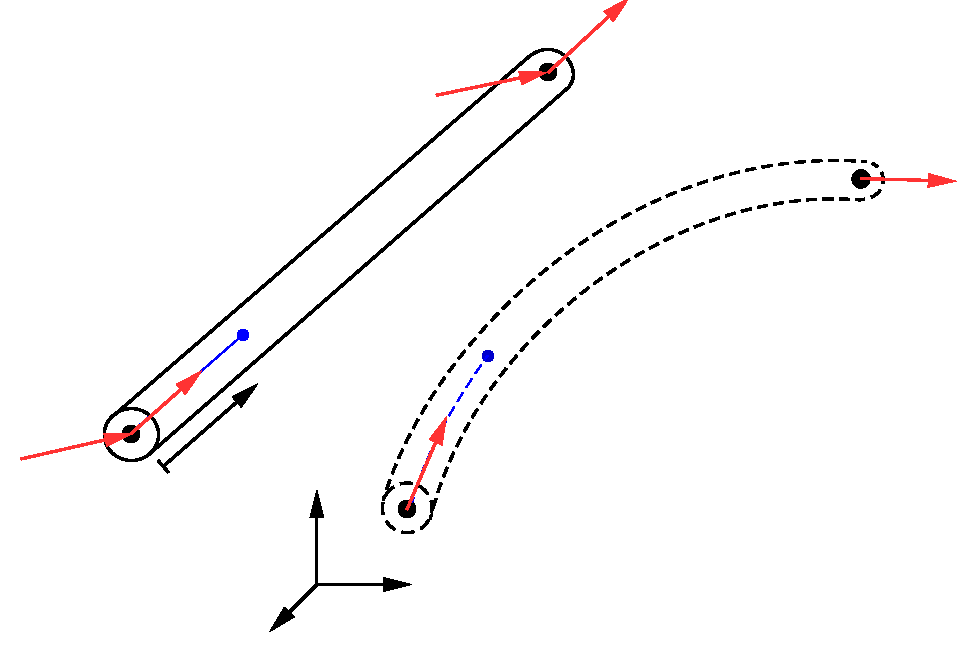
\includegraphics[width=1\textwidth]{images/1dancf.pdf}};
\node at (-5.6,-0.8) {\LARGE $\mathbf{r}^i_x$};
\node at (-7.5,-1.85) {\LARGE $\mathbf{r}^i$};
\node at (-0.6,4.3) {\LARGE $\mathbf{r}^{i+1}$};
\node at (1.8,5.5) {\LARGE $\mathbf{r}_x^{i+1}$};
\node at (-4.2,-2) {\LARGE $\xi$};
\node at (-1.4,-4.8) {\LARGE $X$};
\node at (-3.25,-3.05) {\LARGE $Y$};
\node at (-3.2,-5.35) {\LARGE $Z$};
\node at (-3.8,0) {\LARGE $P$};
\node at (0.35,-0.4) {\LARGE $P$};
\end{tikzpicture}
		\caption{ANCF cable element's schematic. Each node features a global position vector and a position vector gradient along the axis of the element (6DOF). Using shape functions and knowing $\xi$ one can interpolate the degrees of freedom to any point $P$ within the element. } \label{fig:ANCFCable}
\end{figure}
